\section{Methodology}

\subsection{Problem Statement}\label{subsec:problem_Statement}

Accurate discrimination of soft‐tissue types in X‐ray computed tomography (CT) remains a
fundamental challenge in medical imaging. Conventional single‐energy CT produces grayscale
images in which different materials with similar attenuation coefficients (e.g.\,muscle 
vs.\,iodine‐enhanced blood or bone) can appear indistinguishable, leading to diagnostic 
ambiguity. Dual‐energy and photon‐counting CT systems acquire multiple energy‐resolved 
measurements, but extracting robust tissue‐specific maps from these spectral data is 
nontrivial: standard material‐decomposition methods are sensitive to noise, beam‐hardening, 
and detector imperfections, and purely data‐driven deep‐learning approaches often fail to 
generalize beyond their training domain.

This project proposes to address these limitations by developing a \emph{convolutional neural network} 
(CNN) that directly incorporates the known Beer–Lambert attenuation law, $I = I_0 e^{-\mu x}$, and the
two dominant interaction mechanisms—photoelectric absorption and Compton scattering—into its 
architecture. By decomposing each pixel’s dual‐energy attenuation pair \([\mu_{\rm low},\,
\mu_{\rm high}]\) into physically meaningful photoelectric and Compton components and enforcing 
consistency with both the measured attenuation maps and sinogram data, this approach aims to (1)
improve classification accuracy of key tissue types (adipose, fibroglandular, calcification) and (2) 
enhance robustness to noise and out‐of‐distribution scenarios. This integration of first‐principles 
physics with modern deep learning may achieve more reliable, interpretable, and generalizable 
spectral CT tissue characterization.

At the core of this framework is the \emph{U-Net}, a widely used CNN architecture for image segmentation. 
A U-Net consists of a contracting path (encoder) that captures spatial context by progressively 
downsampling feature maps, and an expansive path (decoder) that restores spatial resolution through 
upsampling while combining features from earlier layers via skip connections. This structure enables 
precise, pixel-level predictions while retaining both global context and fine detail.

Two U-Net variants are evaluated in this work:
\begin{itemize}
  \item \textbf{UNet256}: A compact model with \emph{eleven convolutional layers}, including two 
    downsampling blocks and two upsampling blocks. It reduces the input resolution 
    to $128 \times 128$ in the bottleneck layer and is optimized for efficiency and 
    fast inference.
  \item \textbf{UNet512}: A deeper architecture with \emph{fifteen convolutional layers}, 
    incorporating three downsampling and three upsampling stages. It downsamples to $64 \times 64$ 
    in the bottleneck, allowing the network to capture more abstract features and potentially 
    improve segmentation performance for more complex tissue boundaries.
\end{itemize}

By combining these deep learning models with a hybrid loss function—standard binary cross-entropy 
plus a physics consistency penalty—this approach aims to:

\begin{enumerate}
  \item Accurately classify tissue types such as \emph{adipose}, \emph{fibroglandular}, and \emph{calcification};
  \item Enforce consistency with the known physics of spectral CT imaging;
  \item Improve robustness to noise, artifacts, and out-of-distribution samples;
  \item Enable physically grounded, interpretable predictions.
\end{enumerate}

\subsection{Exploratory Data Analysis}\label{sec:exploratory_data_analysis}

The dataset contains 1000 images of ground truth Adipose, Fibroglandular, and Calcification tissue 
maps in the shape $512x512$. Another 1000 cases of low and high $kVp$ transmission data are provided, 
each of which have 256 angle projections onto a linear 1024-pixel detector. Lastly, $kVp$ images
are also provided. These images have pixel dimensions of $512x512$ and are generated from the 
transmission data using Filtered BackProjection (FBP). 

To gain insight into the physical characteristics of the dataset and assess the separability of tissue types in
dual-energy CT space, several visualizations are created that represent a subset of the training data.

\subsubsection{Dual-Energy Scatter Plot}

Figure~\ref{fig:scatter} shows a scatter plot of dual-energy attenuation pairs \([\mu_{\text{low}}, \mu_{\text{high}}]\),
sampled from a volumetric pixels, or voxels, labeled as adipose, fibroglandular, and calcification tissue. Each point corresponds to an
attenuation value at low (50 kVp) and high (80 kVp) energy spectra. Distinct clustering behavior is observed:

\begin{itemize}
    \item \textbf{Adipose} tissue exhibits low attenuation in both energy channels.
    \item \textbf{Fibroglandular} tissue shows intermediate attenuation with greater spread, particularly in the high-energy channel.
    \item \textbf{Calcifications} appear as high-attenuation outliers, especially at low energies due to their dominance of photoelectric interactions.
\end{itemize}

These trends confirm the feasibility of decomposing tissue types based on their dual-energy attenuation signatures.

\begin{figure}[h!]
    \centering
    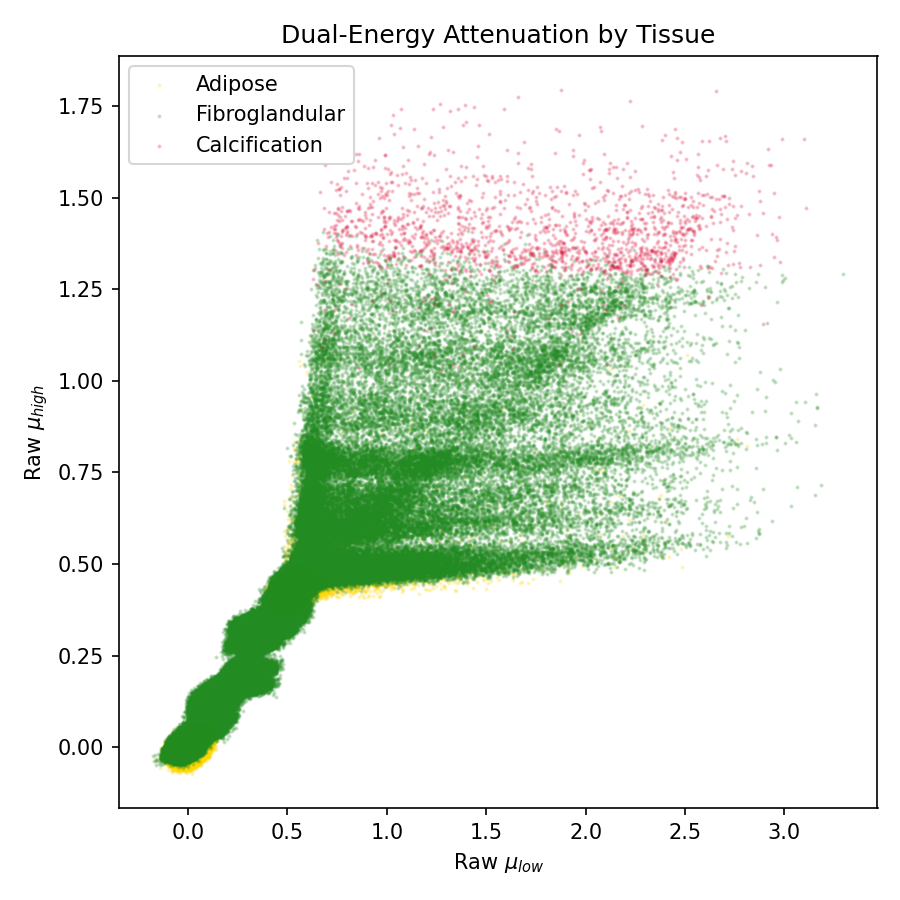
\includegraphics[width=0.5\textwidth]{./fig/attenuation_scatter.png}
    \caption{Dual-energy attenuation scatter plot colored by tissue class.}
    \label{fig:scatter}
\end{figure}

\subsubsection{Energy-Specific Histograms}

Figure~\ref{fig:histograms} presents histograms of attenuation values for each tissue type at low and high energy levels.
These plots illustrate how tissue attenuation shifts between energy spectra due to different interaction mechanisms:

\begin{itemize}
    \item At \textbf{low energy (50 kVp)}, attenuation differences between tissues are more pronounced due to the stronger photoelectric effect.
    \item At \textbf{high energy (80 kVp)}, attenuation values shift downward, reflecting the increased dominance of Compton scattering.
\end{itemize}

These histograms highlight the importance of utilizing both energy channels in modeling tissue properties.

\begin{figure}[h!]
    \centering
    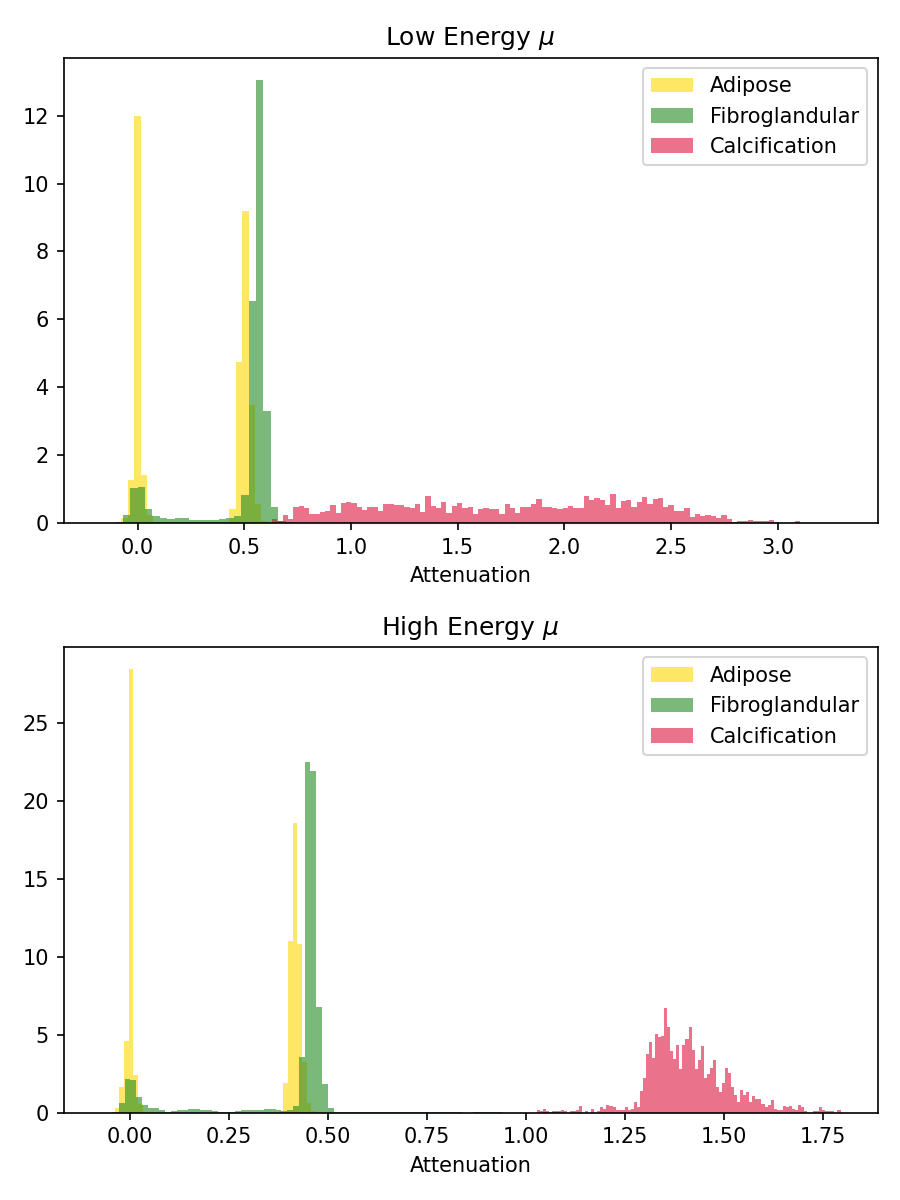
\includegraphics[width=\linewidth]{./fig/attenuation_histograms.png}
    \caption{Histogram of attenuation values by tissue type for low and high energy channels.}
    \label{fig:histograms}
\end{figure}

\subsubsection{Tissue Composition Distribution}

To assess class distribution and tissue prevalence, percentages of each tissue type are computed across all training images. 
The aggregate distributions for adipose, fibroglandular, and calcification tissues are shown in Figure~\ref{fig:composition}. 

\begin{itemize}
    \item \textbf{Adipose} and \textbf{fibroglandular} tissues are well represented, with approximately Gaussian distributions centered around 40\% and 20\%, respectively.
    \item \textbf{Calcification}, however, is does not show up on the figure. Its contribution to each image is typically less than 1\%, making it difficult to visualize 
          on the same scale as the other tissue types. The calcification should be around 0-0.5\% range.
\end{itemize}

As such, a dedicated plot of calcification composition is included in (Figure~\ref{fig:calcification}), which highlights the low prevalence and narrow 
distribution range of this tissue class.

This analysis provides important context for understanding class imbalance, which can impact model calibration and loss sensitivity—especially for 
underrepresented classes like calcifications.

\begin{itemize}
    \item \textbf{Adipose} and \textbf{fibroglandular} tissues are well represented, with Gaussian-like distributions centered around 40\% and 20\%, respectively.
    \item \textbf{Calcification} is relatively rare, typically comprising a small fraction of each image.
\end{itemize}

This analysis provides important context for class imbalance and model calibration.

\begin{figure}[h!]
    \centering
    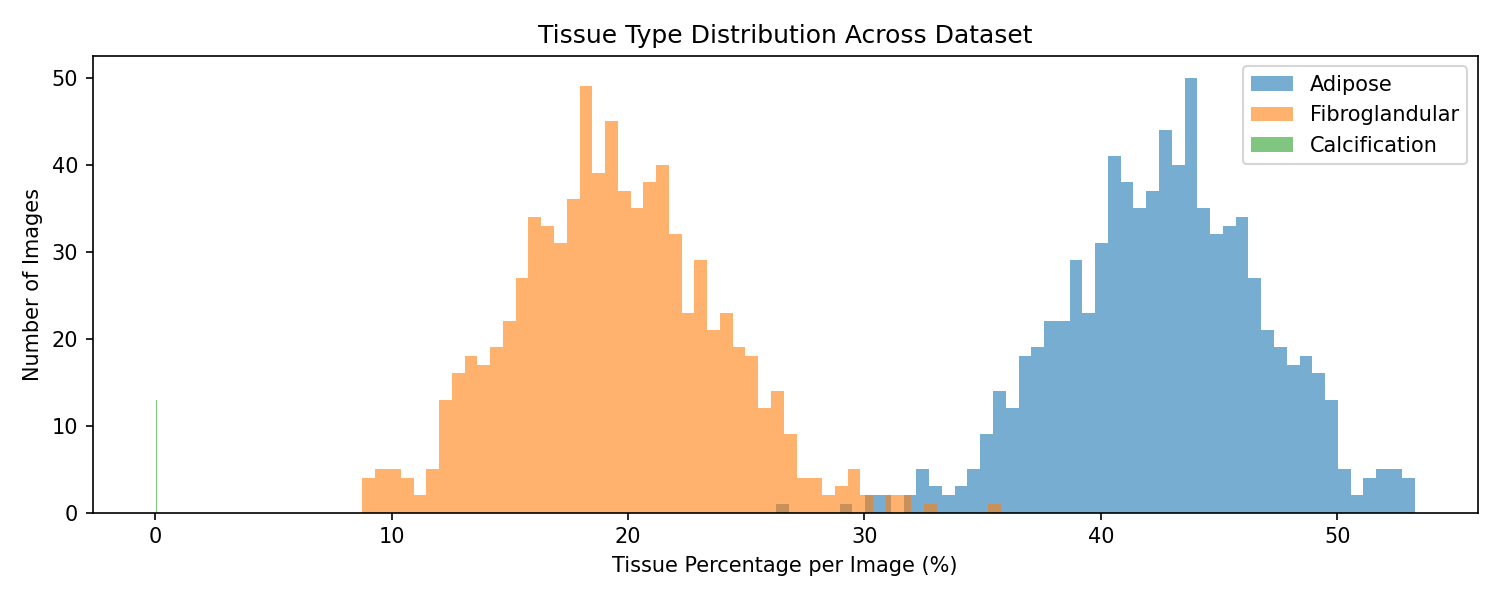
\includegraphics[width=\linewidth]{./fig/tissue_percentage_distribution.png}
    \caption{Distribution of tissue percentages across training images.}
    \label{fig:composition}
\end{figure}

\begin{figure}[h!]
    \centering
    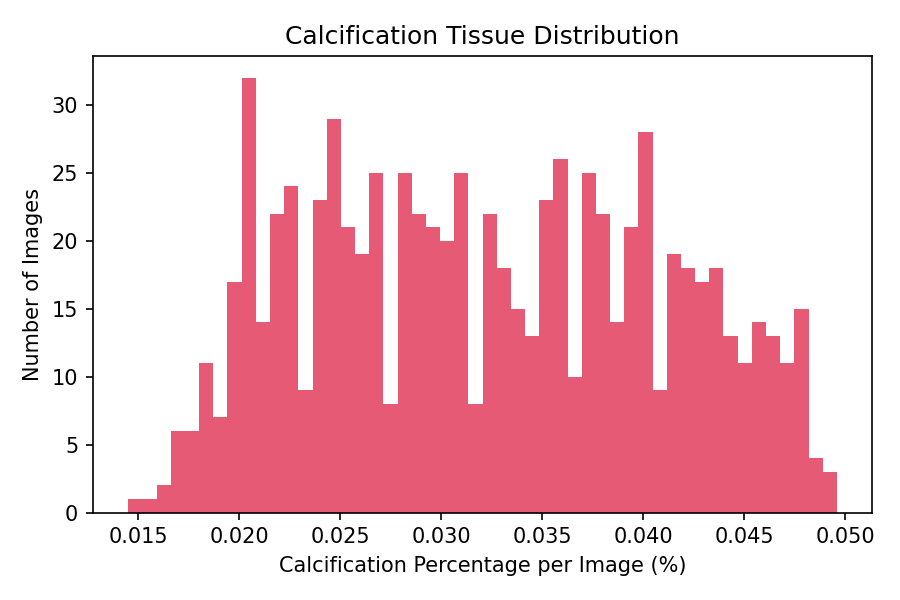
\includegraphics[width=\linewidth]{./fig/calcification_distribution.png}
    \caption{Distribution of calcification percentages across training images. Note the narrow range due to the rare occurrence of calcifications.}
    \label{fig:calcification}
\end{figure}



\subsection{Data Preparation}\label{sec:data_preparation}

The dataset provided by the AAPM~\cite{AAPM2024SpectralCT} includes spectral CT simulation data stored 
in compressed NumPy format. It contains two transmission sinogram datasets, \texttt{lowkVpTransmission} 
and \newline \texttt{highkVpTransmission}, corresponding to 50~kVp and 80~kVp x-ray beams, respectively. These 
datasets represent normalized x-ray transmission values, i.e., the fraction of incident photons that 
pass through the simulated tissue.

Ground truth tissue labels are also provided in the form of binary masks for three tissue types: adipose, 
fibroglandular, and calcification. Each tissue map has the shape $(512 \times 512)$ and identifies the 
true spatial distribution of each class.

To convert the raw transmission data into a form suitable for model training, a custom \texttt{AttnDataset} 
class is created. This class performs the following operations:

\begin{itemize}
    \item Loads the raw sinogram transmission data for low and high energies;
    \item Converts transmission data to attenuation coefficients using the Beer–Lambert law:
    \[
        \mu = -\log(I / I_0),
    \]
    where $I$ is the detected intensity and $I_0$ is assumed to be uniform (1);
    \item Applies filtered back projection (FBP) to reconstruct spatial attenuation maps from sinograms, 
          producing images of shape $(2, 512, 512)$ for each scan, where the two channels correspond to 
          $\mu_{\text{low}}$ and $\mu_{\text{high}}$;
    \item Caches the reconstructed attenuation images as a NumPy array to avoid redundant computation;
    \item Loads the binary ground truth maps for all three tissue types and stacks them into a label array of shape $(3, 512, 512)$;
    \item Splits the dataset into training and test sets using an 80/20 ratio, preserving sample-level consistency.
\end{itemize}

This preprocessing pipeline ensures that each training sample consists of a dual-energy attenuation image and its 
corresponding tissue segmentation mask. The pairing of low and high energy reconstructions facilitates the model's 
ability to learn tissue-specific attenuation patterns driven by both photoelectric and Compton interactions.

\subsection{Models}

This study adopts the U-Net architecture~\cite{ronneberger2015unet}, a widely used convolutional neural network 
(CNN) design for image segmentation tasks. U-Net is particularly well-suited for biomedical applications due to 
its ability to preserve spatial resolution and capture fine-grained features through skip connections between the 
encoder and decoder pathways.

Each U-Net model in this work accepts a 2-channel input image composed of reconstructed low-energy and high-energy 
attenuation maps, \([\mu_{\text{low}}, \mu_{\text{high}}]\), and outputs a 3-channel prediction representing the 
pixelwise likelihoods for \textbf{adipose}, \textbf{fibroglandular}, and \textbf{calcification} tissues.

Two model variants are implemented to assess the effect of network depth and capacity. Both models preserve the 
full-resolution output via upsampling layers and symmetric skip connections, enabling detailed reconstructions 
essential for accurate tissue boundary delineation.

U-Net was chosen over alternatives due to its proven robustness in medical imaging, efficient parameter usage, 
and ability to learn spatial hierarchies across multiple scales—a key advantage when segmenting subtle features 
like low-density calcifications or fibroglandular borders.

\subsubsection{UNet256 and UNet512}

Both \textbf{UNet256} and \textbf{UNet512} are fully convolutional U-Net architectures designed for pixel-wise 
tissue segmentation. Each model takes a dual-channel input—\(\mu_{\text{low}}\) and \(\mu_{\text{high}}\)—representing 
the reconstructed attenuation maps from low and high energy x-rays. The output consists of three channels, corresponding 
to the predicted presence of \textbf{adipose}, \textbf{fibroglandular}, and \textbf{calcification} tissue types at 
each pixel location.

Each encoder stage consists of two sequential 2D convolutional layers (a \textit{ConvBlock}), followed by a 
\(2 \times 2\) max pooling operation to reduce spatial resolution and increase receptive field. A symmetric decoder 
path upsamples the spatial resolution using transposed convolutions, and fuses encoder and decoder features via skip 
connections to recover fine-grained spatial detail.

\begin{itemize}
    \item \textbf{UNet256} employs two encoding stages with feature dimensions expanding from 2 to 64 and then 128, 
          followed by a bottleneck layer of 256 channels at \(128 \times 128\) resolution. It then decodes back up 
          through two symmetric stages to produce a final \(3 \times 512 \times 512\) prediction map.
    \item \textbf{UNet512} adds a third encoding stage, extending the channel depth from 128 to 256 before reaching a 
          bottleneck of 512 channels. Like UNet256, it downsamples to \(128 \times 128\), but includes three decoder 
          blocks, enabling the network to capture richer features and more complex tissue boundaries.
\end{itemize}

This architecture choice strikes a balance between learning expressivity and spatial precision, making it well suited to 
the challenges of spectral CT tissue decomposition.
